\documentclass[a4paper,11pt]{article}

\usepackage{amsmath}
\usepackage{amssymb}

% for proofs  environment
\usepackage{amsthm}

\usepackage[backend=bibtex]{biblatex}
\bibliography{slides5b}

% for probability trees
\usepackage{tikz}
\usetikzlibrary{trees}

% for plots
\usepackage{ pgfplots}
% inserted on suggestion in warning during compilation
\pgfplotsset{compat=1.9}

%for strikethrough text
\usepackage{soul}

%for R source code listing
\usepackage{listings}

%for block quotes
\usepackage{csquotes}

% for including images
\usepackage{graphicx}
\graphicspath{{.}}

% For not indenting the first line of paragraphs:
\setlength{\parindent}{0pt}
% define the title
\author{John Hancock}
\title{MIT Introduction to Statistics 18.05 - answers to questions in second class 5 }
\begin{document}
% generates the title
\maketitle
% insert the table of contents
\tableofcontents
\section{References and License}
We are answering questions in the material from MIT OpenCourseWare
course 18.05, Introduction to Probability and Statistics.

In this document we are answering questions Orloff and Bloom ask in
\cite{slides5b}.

We use documentation in \cite{includeGr} to write the \LaTeX source code for
this document.

Please see the references section for detailed citation information.

The material for the course is licensed under the terms at
\url{http://ocw.mit.edu/terms}.

We use documentation in
to write \LaTeX source code for this document.

\section{Probability within distances from the mean}

\subsection{ $\mu = 0$, $\sigma=1$}
In \cite{reading5c} Orloff and Bloom state that for the continuous random
variable $Z \sim N \left(0, 1 \right)$:
\begin{itemize}
	\item $P\left( -1 \leq Z \leq 1 \right) \approx 0.68$
	\item $P\left( -2 \leq Z \leq 2 \right) \approx 0.95$
	\item $P\left( -3 \leq Z \leq 3 \right) \approx 0.99$
\end{itemize}

\subsection{ $\mu=0$, $\sigma=3$}

Orloff and Bloom ask a question similar to the previous, but change the
standard deviation of the distribution to 3.

We use R to compute how much probability is within $\sigma$ of $\mu$, $2\sigma$
of $\mu$, and $3\sigma$ of $\mu$

\begin{lstlisting}
	> pnorm(3, 0, 3) - pnorm(-3, 0, 3)
[1] 0.6826895
> pnorm(6, 0, 3) - pnorm(-6, 0, 3)
[1] 0.9544997
> pnorm(9, 0, 3) - pnorm(-9, 0, 3)
[1] 0.9973002
\end{lstlisting}

Interestingly enough, these are the same results as for the normal distribution
with mean 0 and standard deviation 1.

Next, Orloff and Bloom ask us if changing $\mu$ changes our answer to problem
2.  Indeed it does.  We use the pnorm function in R to see how the answer
changes when we set $\mu = 10$:

\begin{lstlisting}
	> pnorm(3, 10, 3) - pnorm(-3, 10, 3)
[1] 0.009807985
> pnorm(6, 10, 3) - pnorm(-6, 10, 3)
[1] 0.09121117
> pnorm(9, 10, 3) - pnorm(-9, 10, 3)
[1] 0.3694413
\end{lstlisting}

\section{Histogram of exp$\left(1 \right)$ random variable}

We make a small modification to the code in \cite{studio3r} to plot a histogram
of $1,000$ sambles of a random variable that follows an exp$\left(1 \right)$
distribution:

\begin{lstlisting}
data = rexp(1000,1)
binwidth = .4
bins = seq(min(data), max(data)+binwidth, binwidth)
hist(data, breaks=bins, col='purple')
\end{lstlisting}

We run this code in RStudio to produce the following graphic:

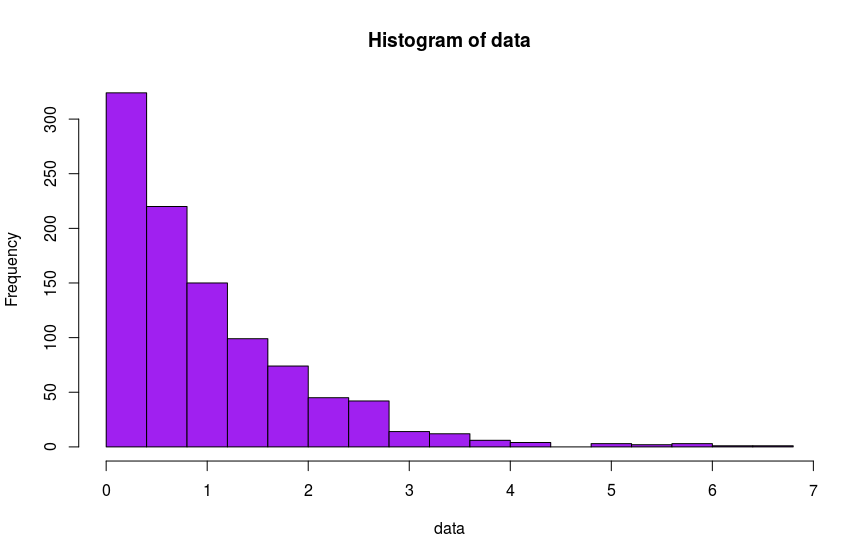
\includegraphics[scale=0.5]{histogram-exp-1}

\section{Histogram of average of 2 exp$\left(1 \right)$ random variables}

Orloff and Bloom ask us to draw a histogram of the average of two independent
variables that follow the exp$\left( 1 \right)$ distribution.

We make a small modification to the code in \cite{studio3r} to draw the
histogram.  We run the following code in RStudio:

\begin{lstlisting}
data = (rexp(1000,1) + rexp(1000,1))/2
binwidth = .4
bins = seq(min(data), max(data)+binwidth, binwidth)
hist(data, breaks=bins, col='purple', freq=FALSE)
\end{lstlisting}

To produce this histogram:

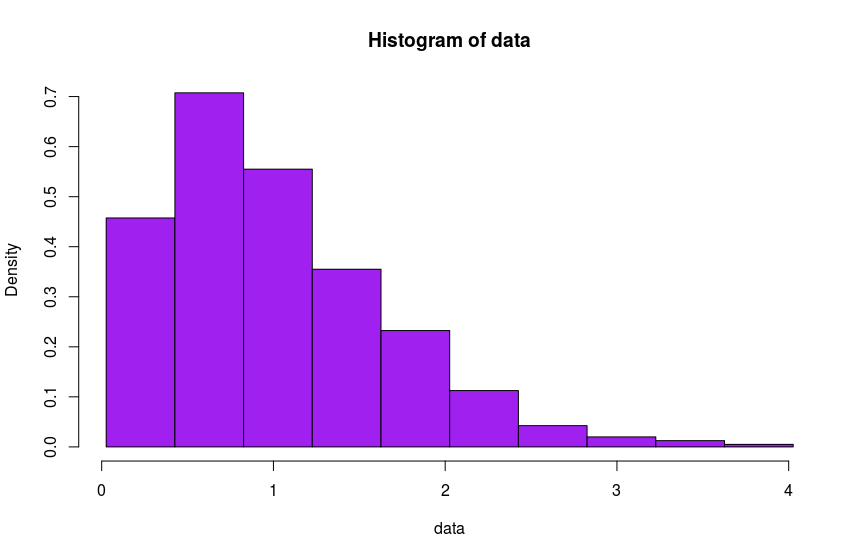
\includegraphics[scale=0.5]{hist-2-exp-1}

\section{Histogram of 50 exp$\left(1 \right)$ random variables}

We make another modificaiton to the R code that Orloff and Bloom give us in
\cite{studio3r} to plot the histogram.  We run the code here:
\begin{lstlisting}
data = colMeans(matrix(rexp(50*10000), 50, 10000))
binwidth = .1
bins = seq(min(data), max(data)+binwidth, binwidth)
hist(data, breaks=bins, col='purple', freq=FALSE)
\end{lstlisting}

To produce this histogram
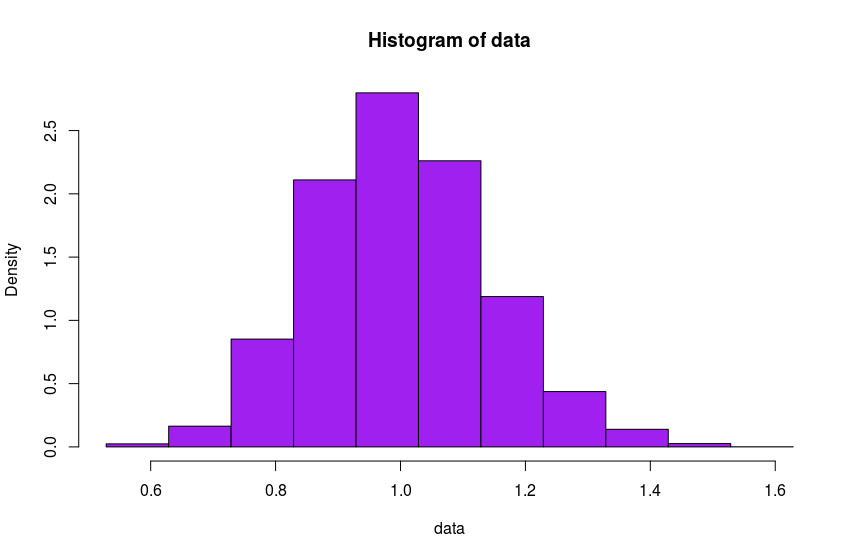
\includegraphics[scale=0.5]{hist-50-exp}

\section{Superimpose plot of normal distribution}

This is our attempt to superimpose a plot of the normal distribution
$N\left( 1, \frac{1}{50}\right)$.

We modify code in \cite{studio3r}:
\begin{lstlisting}
	data = colMeans(matrix(rexp(50*10000), 50, 10000))
binwidth = .1
bins = seq(min(data), max(data)+binwidth, binwidth)
hist(data, breaks=bins, col='purple', freq=FALSE)
x = seq(0,max(data)+1,.01)
lines(x,rnorm(x,1/50), col='red', lwd=4)
\end{lstlisting}

We run this code in RStudio to produce the following graphic:

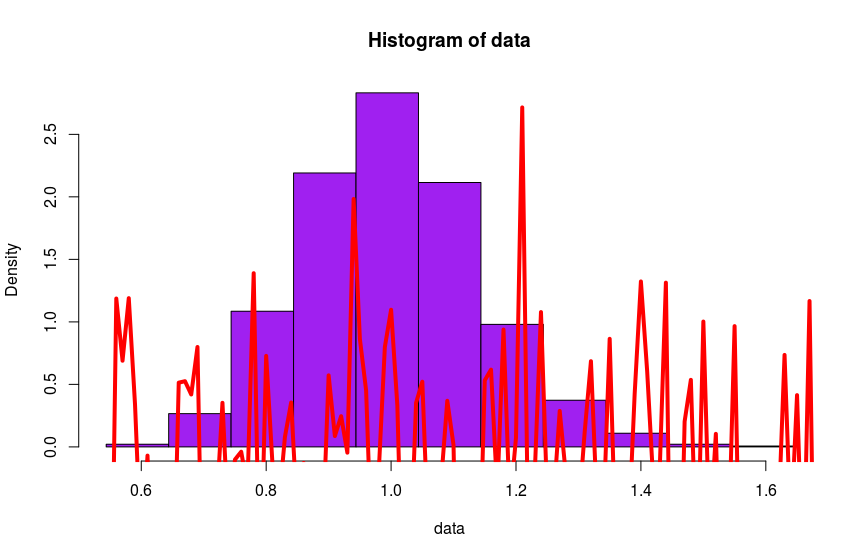
\includegraphics[scale=0.5]{superimpose}

\printbibliography{}
\end{document}
